\documentclass[fleqn,10pt]{wlscirep}
\usepackage[utf8]{inputenc}
\usepackage[T1]{fontenc}

\newcommand{\james}[1]{\noindent{\textcolor{blue}{\textbf{ James:} \textsf{#1} }}}
\newcommand{\ashley}[1]{\noindent{\textcolor{orange}{\textbf{ Ashley:} \textsf{#1} }}}
\newcommand{\anie}[1]{\noindent{\textcolor{red}{\textbf{ Allen:} \textsf{#1} }}}

\newcommand{\edit}[1]{\textcolor{black}{#1}}
\newcommand{\newedit}[1]{\textcolor{black}{#1}}

\setlength{\paperwidth}{21cm}   % A4
\setlength{\paperheight}{29.7cm}% A4
\setlength\topmargin{-0.5cm}
\setlength\oddsidemargin{0cm}   
\setlength\textheight{24.7cm} 
\setlength\textwidth{16.5cm}
\setlength\columnsep{0.6cm}  
% \setlength\columnwidth{}

% custom packages
\usepackage{subcaption}
\usepackage{bm}
\usepackage{csquotes}
\usepackage{framed}
\usepackage{multicol}
\usepackage{amsmath}
\usepackage{changepage}
\usepackage{multirow}
\usepackage{setspace}

%% Include all macros below

\newcommand{\dataset}{{\cal D}}
\newcommand{\fracpartial}[2]{\frac{\partial #1}{\partial  #2}}

\def\E{\mathbb{E}} % Expectation symbol
\def\Gsn{\mathcal{N}} % Normal distribution symbol
\def\Cov{\mrm{Cov}} % Covariance symbol
\def\reals{\mathbb{R}}
\newcommand{\capital}[1]{\bm{\mathrm{#1}}}
\renewcommand{\exp}[1]{\operatorname{exp}\left(#1\right)} % Exponential
\DeclareMathOperator*{\argmax}{argmax}
\DeclareMathOperator*{\argmin}{argmin}
\def\indic#1{\mbb{I}\left({#1}\right)} % Indicator function
\def\indicsub#1#2{\mbb{I}_{#2}\left({#1}\right)} % Indicator function

% TODO:
% 1. No footnote! 

\title{DeepTag: inferring diagnoses from veterinary clinical notes}

\author[1,+]{Allen Nie}
\author[1,+]{Ashley Zehnder}
\author[2]{Rodney L. Page}
\author[3]{Yuhui Zhang}
\author[1]{Arturo Lopez Pineda}
\author[1]{Manuel A. Rivas}
\author[1,4]{Carlos D. Bustamante}
\author[1,4, *]{James Zou}
\affil[1]{Department of Biomedical Data Science, Stanford University, Stanford, CA 94305, USA}
\affil[2]{Department of Clinical Sciences, Colorado State University, Fort Collins, CO 80523, USA}
\affil[3]{Department of Computer Science and Technology, Tsinghua University, Beijing, China}
\affil[4]{Chan-Zuckerberg Biohub, San Francisco, CA 94158, USA}

\affil[+]{these authors contributed equally to this work}
\affil[*]{Corresponding author. jamesz@stanford.edu}

\begin{abstract}
Large scale veterinary clinical records can become a powerful resource for patient care and research. However, clinicians lack the time and resource to annotate patient records with standard medical diagnostic codes and most veterinary visits are captured in free text notes. The lack of standard coding makes it challenging to use the clinical data to improve patient care. 
It is also a major impediment to cross-species translational research, which relies on the ability to accurately identify patient cohorts with specific diagnostic criteria in humans and animals. In order to reduce the coding burden for veterinary clinical practice and aid translational research, we have developed a deep learning algorithm, DeepTag, which automatically infers diagnostic codes from veterinary free text notes. DeepTag is trained on a newly curated dataset of 112,558 veterinary notes manually annotated by experts.
DeepTag extends multi-task LSTM with an improved hierarchical objective that captures the semantic structures between diseases. To foster human-machine collaboration, DeepTag also learns to abstain in examples when it is uncertain and defers them to human experts, resulting in improved performance. DeepTag accurately infers disease codes from free text even in challenging cross-hospital settings where the text comes from different clinical settings than the ones used for training. It enables automated disease annotation across a broad range of clinical diagnoses with minimal pre-processing. The technical framework in this work can be applied in other medical domains that currently lack medical coding resources.
\end{abstract}
\begin{document}

\flushbottom
\maketitle

\thispagestyle{empty}

% \noindent Please note: Abbreviations should be introduced at the first mention in the main text – no abbreviations lists. Suggested structure of main text (not enforced) is provided below.

% \doublespacing
\onehalfspacing

\section*{Introduction}

While a robust medical coding infrastructure exists in the US healthcare system for human medical records, this is not the case in veterinary medicine, which 
 lacks coding infrastructure and standardized nomenclatures across medical institutions. Most veterinary clinical notes are not coded with standard SNOMED-CT diagnosis~\cite{o2014approaches}. 
This hampers efforts at clinical research and public health monitoring. Due to the relative ease of obtaining large volumes of free-text veterinary clinical records for research (compared to similar volumes of human medical data) and the importance of turning these volumes of text into structured data to advance clinical research, we investigated effective methods for building automatic coding systems for the veterinary records. 

It is becoming increasingly accepted that spontaneous diseases in animals have important translational impact on the study of human disease for a variety of disciplines \cite{kol2015companion}. Beyond the study of zoonotic diseases, which represent 60-70\% of all emerging diseases, non-infectious diseases, like cancer, have become increasingly studied in companion animals as a way to mitigate some of the problems with rodent models of disease \cite{leblanc2015defining}. Additionally, spontaneous models of disease in companion animals are being used in drug development pipelines as these models more closely resemble the ``real world'' clinical settings of diseases than genetically altered mouse models~\cite{grimm2016bark,klinck2017translational,baraban2014new,hernandez2018naturally}. 
However, when it comes to identifying clinical cohorts of veterinary patients on a large scale for clinical research, there are several problems.  One of the first is that veterinary clinical visits rarely have diagnostic codes applied to them, either by clinicians or medical coders.  There is no substantial third party payer system and no HealthIT act that applies to veterinary medicine, so there are few incentives for clinicians or hospitals to annotate their records for diseases to be able to identify patients by diagnosis.  Billing codes are largely institution-specific and rarely applicable across institutions, unless hospitals are under the same management structure and records system. Some large corporate practice groups have their own internal clinical coding structures, but that data is rarely made available for outside researchers. A small number ($< 5$) academic veterinary centers (of a total of 30 veterinary schools in the US) employ dedicated medical coding staff that apply disease codes to clinical records so these records can be identified for clinical faculty for research purposes. How best to utilize this rare, well-annotated, veterinary clinical data for the development of tools that can help organize the remaining seqments of the veterinary medical domain is an open area of  research. 

In this paper, we develop DeepTag, a system to automatically code veterinary clinical notes. DeepTag takes free-form veterinary note as input and infers clinical diagnosis from the note. The inferred diagnosis is in the form of 42 SNOMED-CT codes. We trained DeepTag on a large set of 112,558 veterinary notes, and each note is expert labeled with a set of SNOMED-CT codes. DeepTag is a bidirectional long-short term memory network (BLSTM) augmented with a hierarchical training objective that captures similarities between the diagnosis codes. We evaluated DeepTag's performance on challenging cross-hospital coding tasks.

Natural language processing (NLP)  techniques have improved from leveraging discrete patterns such as n-grams \cite{jurafsky2014speech} to continuous learning algorithms like Long-short-term Memory Networks (LSTMs) \cite{hochreiter1997long}. This strategy has proven to be very successful when a sizable amount of data can be acquired. Combined with advances in optimization and classification algorithms, the field has developed algorithms that can match or exceed human performance in several traditionally difficult tasks \cite{goldberg2017neural}.

Analyzing free text such as diagnostic reports and clinical notes has been a central focus of clinical natural language processing~\cite{velupillai2015recent}. Most of the previous research has focused on the human healthcare systems. Examples include using NLP tools to improve pneumonia screening in the emergency department, assisting in adenoma detection, assisting and simplifying hospital processes by identifying billing codes from clinical notes~\cite{demner2016aspiring}. Pivovarov et al. have conducted experiments to discover phenotypes and diseases using an unsupervised method on a broad set of heterogeneous data~\cite{pivovarov2015learning}.

In the domain of veterinary medicine, millions of clinical summaries are stored as electronic health records (EHR) in various hospitals and clinics. Unlike human discharge summaries that have been assigned with billing codes (ICD-9/ICD-10 codes), veterinary summaries exist primarily as free text. This makes it challenging to perform  systematic analysis  such as disease prevalence studies, analysis of adverse drug effects, therapeutic efficacy or outcome analysis. Veterinary domain is very favorable for an NLP system that can convert large amount of  free-text notes into structured information. Such a system would benefit the veterinary community in a substantial way and can be deployed in multiple clinical settings. Veterinary medicine is a domain where clinical NLP tools can have a substantial impact in practice and be integrated into daily use.

Identifying a set of conditions/diseases from clinical notes has been actively studied~\cite{demner2016aspiring,lipton2015learning}. Currently, the task of transforming free text into structured information primarily relies on two approaches: named entity recognition (NER) and automated coding. DeepTag is designed to perform automated coding rather than NER. NER requires annotation on the word level, where each word is associated with one of a few types. In the ShARe task \cite{pradhan2014evaluating}, the importance is placed on identifying disease span and then normalizing into standard terminology in SNOMED-CT or UMLS (Unified Medical Language System). In other works, the focus has been on tagging each word with a specific type: adverse drug effect, severity, drug name, etc~\cite{jagannatha2016bidirectional}. Annotating on word level is expensive, and most corpora contain only a couple of hundreds or thousands of clinical notes. Even though early shared task in this domain has proven to be successful  ~\cite{pradhan2014semeval,elhadad2015semeval}, it is still difficult to curate a large dataset in this manner.

Automated coding on the other hand takes the entire free text as input, and infers a set of codes that are used to code the entire work. Most discharge summaries in human hospitals have billing codes assigned. Baumel et al. proposed a text processing model for automated coding that processes each sentence first and then processes the encoded hidden states for the entire document~\cite{baumel2017multi}.This multi-level approach is especially suitable for longer texts, and the method was applied to the MIMIC data, where each document is on average five times longer than the veterinary notes from CSU. Rajkomar et al. used deep learning methods to process the entire EHR and make clinical predictions for a wide range of problems including automated coding~\cite{rajkomar2018scalable}. In their work, they compared three deep learning models: LSTM, time-aware feedforward neural network (TANN), and boosted time-based decision stumps. In this work, we use a new hierarchical training objective which is designed to capture the similarities among the SNOMED-CT codes. This hierarchical objective is complementary to these previous approaches in the sense that the hierarchical objective can be used on top of any architecture. Our cross-hospital evaluations also extend what is typically done in literature. Even though Rajkomar et al. had data from two hospitals, they did not investigate the performance of the model when trained on one hospital but evaluated on the other. In our work, due to the lack of coded clinical notes in the veterinary community beyond a few academic hospitals, it is especially salient for us to evaluate the model’s ability to generalize across hospitals.

Our work is also related to the work of Kavuluru et al., who experimented with different training strategies and compared which strategy is the best for automated coding~\cite{kavuluru2015empirical}, and Subotin et al., who improved upon direct label probability estimation and used a conditional probability estimator to fine-tune the label probability~\cite{subotin2016method}. Perotte et al. also investigated possible methods to leverage the hierarchical structure of disease codes by using an SVM algorithm on each level of the ICD-9 hierarchy tree~\cite{perotte2013diagnosis}.

Cross-hospital generalization is a significant challenge in the veterinary coding setting. Most veterinary clinics currently do not apply diagnosis codes to their notes~\cite{o2014approaches}. Therefore our training data can only come from a handful of university-based regional referral centers that manually code their free text notes. The task is to train a model on such data and deploy for thousands of private hospitals and clinics. University-based centers and private hospitals and clinics have substantial variation in the writing style, the patient population, and the distribution of diseases (Figure~\ref{fig:csu-pp-text-examples}). For example, the training dataset we have used in this work comes from a university-based hospital with a high-volume referral oncology service, but typical local hospitals might face more dermatologic or gastrointestinal cases.

\section*{Results}

DeepTag takes clinician's notes as input and predicts a set of SNOMED-CT disease codes. SNOMED-CT is a comprehensive and precise clinical health terminology managed by the International Health Terminology Standards Development Organization. DeepTag is a bi-directional long short-term memory (LSTM) neural network with a new hierarchical learning objective designed to
capture similarities between the disease codes (see Supplementary Materials for model details). 

DeepTag is trained on 112,558 annotated veterinary notes from the Colorodo State University of Veterinary Medicine and Biomedical Sciences (CSU) curated for research purposes. Each of these notes is a free text description of a patient visit, and is manually tagged with at least one, and on average eight, out of the 41 SNOMED-CT disease codes by experts. 
In addition, we map every non-disease related code to an extra  code. In total, DeepTag learns to tag a clinical note with a subset of 42 codes.
 
We evaluate DeepTag on two different datasets. One consists of 5,628 randomly sampled non-overlapping held-out documents from the same CSU dataset that the system is trained on. The other dataset contains 586 documents and are collected from a private practice (PP) located in northern California. Each of the these document is also manually annotated with the appropriate SNOMED-CT codes by human experts. We refer to this dataset as the PP dataset. 

We regard the PP dataset as a ``out-of-domain'' dataset due to its substantial difference with regard to writing style and institution type compared to the CSU dataset~\cite{li2012literature}. The PP documents tend to be substantially shorter (average of 253 words compared to 368 words in CSU), use more abbreviations and have different distribution of diseases (see Methods section for more details).
 
\subsection*{Tagging performance}

We present DeepTag's performance on the CSU and PP test data in Table~\ref{tab:detailed-csu-pp}. To save space, we display the 20 most frequent disease codes in Table~\ref{tab:detailed-csu-pp}. For each disease code, we report the number of training examples for the disease code ($N$), the scores for precision, recall, $F_1$, ROC AUC, and the number of subtypes in this disease code. While DeepTag achieves reasonable $F_1$ scores overall, its performance is quite heterogeneous for different disease codes. Moreover, the performance decreases when DeepTag is applied to the out-of-domain PP test data. 
We identify two factors that substantially impact DeepTag's performance: 1) the number of training examples that are tagged with the given disease code; 2) the number of subtypes, where a subtype is a SNOMED-CT code applied to either dataset that is lower in the SNOMED-CT hierarchy than the top-level disease codes DeepTag is predicting. We use the number of subtypes as a proxy for the diversity and specificity of the clinical text descriptions. Thus, a higher number of subtypes suggests a wider spectrum of diseases.

\section*{Discussion}

The Discussion should be succinct and must not contain subheadings.

\section*{Methods}

Topical subheadings are allowed. Authors must ensure that their Methods section includes adequate experimental and characterization data necessary for others in the field to reproduce their work.

\bibliography{sample}

\section*{Acknowledgements (not compulsory)}

Acknowledgements should be brief, and should not include thanks to anonymous referees and editors, or effusive comments. Grant or contribution numbers may be acknowledged.

\section*{Author contributions statement}

Must include all authors, identified by initials, for example:
A.A. conceived the experiment(s),  A.A. and B.A. conducted the experiment(s), C.A. and D.A. analysed the results.  All authors reviewed the manuscript. 

\clearpage

\section*{Supplementary Materials}

\subsection*{Supplementary Figures}

% To include, in this order: \textbf{Accession codes} (where applicable); \textbf{Competing interests} (mandatory statement). 

% The corresponding author is responsible for submitting a \href{http://www.nature.com/srep/policies/index.html#competing}{competing interests statement} on behalf of all authors of the paper. This statement must be included in the submitted article file.

\begin{figure*}[h!]
    \begin{subfigure}[b]{\textwidth}
        \centering
        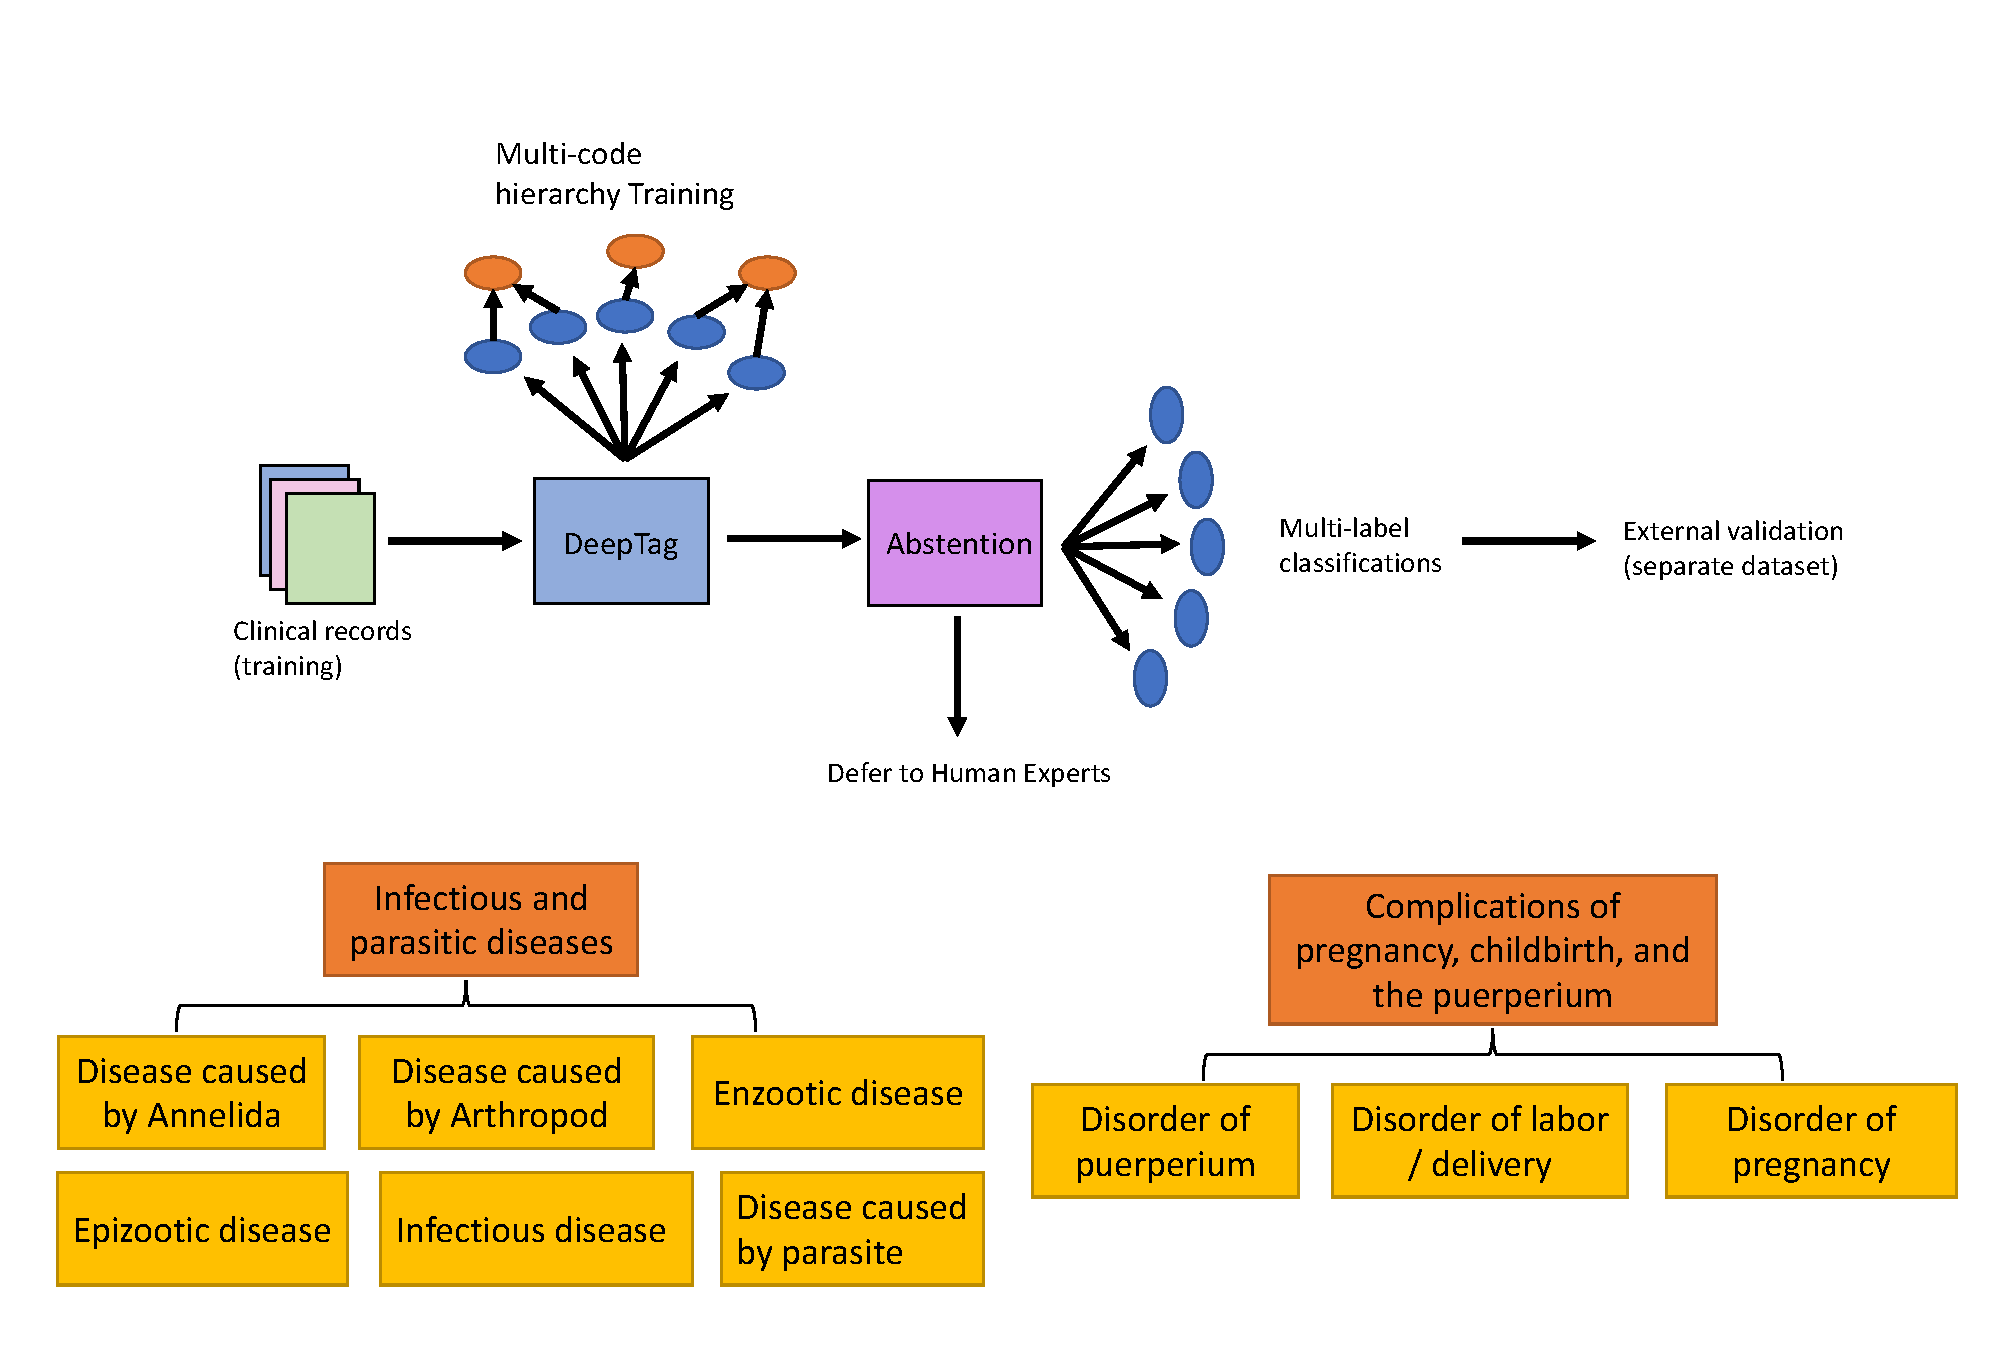
\includegraphics[scale=0.4]{combined-figure-1.pdf}
        \caption{}
        \label{fig:work-schematic}
    \end{subfigure}
    \hfill
    \begin{subfigure}[b]{\textwidth}
        \footnotesize
        \textbf{CSU clinical note example}
        \begin{framed}
        Jem is a 10 year old male castrated hound mix that was presented for continuation of chemotherapy for previously diagnosed B-cell multicentric lymphoma. Jem was started on CHOP chemotherapy last week and has been doing very well since receiving doxorubicin. The owners have noted his lymph nodes have gotten much smaller. He has some loose stool, yet improved with metronidazole. Current medications include prednisolone. Assessment: Jem is in a strong partial remission based on today's physical exam. He is also doing very well since starting chemotherapy. A CBC today was unremarkable and adequate for chemotherapy. She was dispensed oral cyclophosphamide and furosemide that the owners were instructed to give at home.
        \vspace{0.1in}
        
        \textbf{Expert annotated diseases}: Disorder of hematopoietic cell proliferation, Neoplasm and/or hamartoma
        % Disease codes: Disorder of hematopoietic cell proliferation(28), Neoplasm and/or hamartoma(40)
        \end{framed}
        
        \textbf{Private practice (PP) clinical note example}
        \begin{framed}
        Likely ear infection  shaking head  now swollen  drooping ear otherwise doing well  amublating well- had RF carpal arthrodesis at UCD. wt:  95.3 lbs.    Ears/Eyes/Nose/Throat: Clear OU/ brown yeasty debris AU errythema AU no fb/tm;s intact AU mod aural hematoma AD  Cardiovascular:   No murmur/arrhythmia.  Femoral pulses strong and synchronous. HR:84  Respiratory:  Lungs sound clear bilaterally  no crackles or wheezes. Eupneic.  RR:20  Lymph nodes:   No palpable peripheral lymphadenopathy  Oral Exam:  mm pink and moist.   CRT $<$ 2 sec  Musculoskeletal:  No lameness noted. Arthrodesis carpal joint RF  thickened stifle LH  ambulating well  Nervous System:   Appropriate mentation.  No overt neurologic deficits  Integument:  Full haircoat. Adequate skin turgor. otitis externa AU  aural hematoma AD. Ear cytology -  ++cocci  yeast   AU.  Cleaned  with epiotic. Rx Tresaderm BID x  14 days.  applied first dose    Rx temarilP taper    Skin prep medial AD over hematoma.  then 19g butterfly needle attached to syringe  drained 10ml bloody fluid  held pressure with guaze  no more bleeding        CE: Recheck in 14d to ensure infection cleared  discussed aural hematomas  options for tx  sx. may recur. 
        \vspace{0.1in}
    
        \textbf{Expert annotated diseases}: Infectious disease, Disorder of the integument, Disorder of the auditory system
        \end{framed}
        \caption{}
        \label{fig:csu-pp-text-examples}
    \end{subfigure}
    \caption{{\bf System workflow and clinical note examples.} Figure (a) shows  the workflow of DeepTag  with abstention. Then we show two example meta-diseases corresponding to two subsets of the 42 SNOMED-CT codes. Figure (b) shows two example notes from the CSU and PP datasets. }
    \label{fig:figure1}
\end{figure*}

\begin{figure}[!h]
\centering
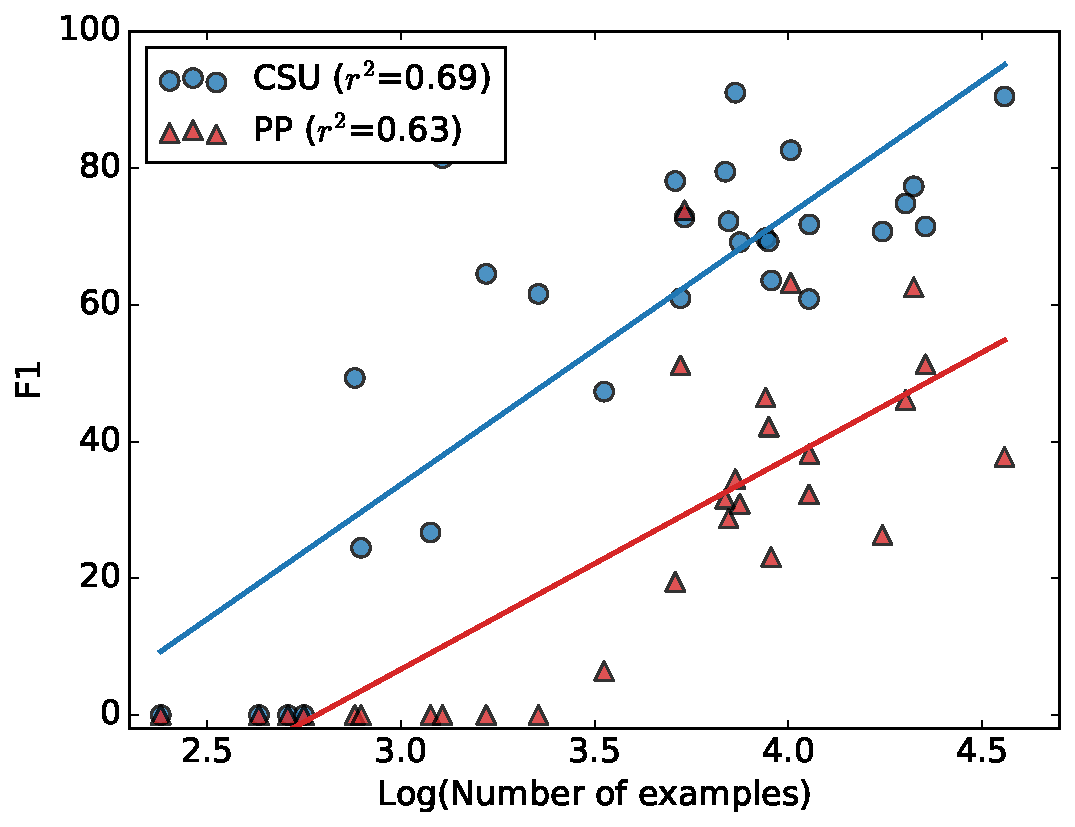
\includegraphics[scale=0.4]{example_f1_scatterplot.pdf}
\caption{{\bf Per-disease code $F_1$ score plotted with log of number of examples in the training dataset.} Results shown here are from the DeepTag model. Each point represents a disease code, its corresponding number of training examples in CSU, and the per-disease code $F_1$ score from the DeepTag model.
}
\label{fig:example-f1-scatterplot}
\end{figure}

\clearpage

\subsection*{Supplementary Tables}

\begin{table*}[h]
\centering
\footnotesize
\begin{adjustwidth}{-0.5in}{0in}
\caption{\textbf{Report of DeepTag performance on the CSU test data and PP data}}
\begin{tabular}{c | c c c c c c | c c c c c c }
\toprule
 & \multicolumn{6}{c|}{CSU} & \multicolumn{6}{c}{PP (\edit{Cross-hospital})}  \\
\newedit{Disease code} & \edit{N} & Prec & Rec & $F_1$ & \newedit{AUC} & Sub & \edit{N} & Prec & Rec & $F_1$ & \newedit{AUC}  & Sub \\
\midrule
Autoimmune disease  & 1280 & 94.0 & 72.3 & 81.4 & \newedit{0.86} & 11 & 1 & 0.0 & 0.0 & 0.0 & \newedit{0.50} & 1(1) \\ 
Congenital disease  & 3345 & 72.9 & 35.9 & 47.3 & \newedit{0.68} & 224 & 17 & 46.7 & 3.5 & 6.4 & \newedit{0.52} & 8(6) \\ 
Propensity to adverse reactions  & 5105 & 89.1 & 70.2 & 78.1 & \newedit{0.85} & 8 & 43 & 67.2 & 12.6 & 19.5 & \newedit{0.56} & 7(2) \\ 
Metabolic disease  & 5265 & 68.9 & 55.4 & 61.0 & \newedit{0.77} & 82 & 26 & 56.6 & 48.5 & 51.1 & \newedit{0.73} & 12(9) \\ 
Disorder of auditory system  & 5393 & 81.0 & 66.2 & 72.8 & \newedit{0.83} & 67 & 64 & 78.8 & 70.3 & 73.8 & \newedit{0.84} & 12(6) \\ 
Hypersensitivity condition  & 6871 & 85.7 & 74.6 & 79.5 & \newedit{0.87} & 31 & 50 & 67.7 & 22.4 & 31.6 & \newedit{0.61} & 11(4) \\ 
Disorder of endocrine system  & 7009 & 79.2 & 66.7 & 72.2 & \newedit{0.83} & 84 & 46 & 44.4 & 21.7 & 28.7 & \newedit{0.60} & 8(8) \\ 
Disorder of hematopoietic cell proliferation  & 7294 & 95.1 & 87.4 & 91.0 & \newedit{0.94} & 22 & 16 & 62.7 & 25.0 & 34.5 & \newedit{0.62} & 6(1) \\ 
Disorder of nervous system  & 7488 & 76.1 & 63.8 & 69.2 & \newedit{0.81} & 243 & 27 & 40.4 & 26.7 & 30.8 & \newedit{0.62} & 19(14) \\ 
Disorder of cardiovascular system  & 8733 & 79.3 & 62.5 & 69.7 & \newedit{0.81} & 351 & 53 & 44.1 & 52.1 & 46.4 & \newedit{0.73} & 30(24) \\ 
Disorder of the genitourinary system  & 8892 & 77.7 & 62.6 & 69.3 & \newedit{0.81} & 317 & 44 & 47.8 & 39.1 & 42.2 & \newedit{0.68} & 19(12) \\ 
Traumatic AND/OR non-traumatic injury  & 9027 & 72.8 & 57.2 & 63.5 & \newedit{0.78} & 536 & 19 & 50.5 & 15.8 & 23.1 & \newedit{0.58} & 13(8) \\ 
Visual system disorder  & 10139 & 84.3 & 81.1 & 82.6 & \newedit{0.90} & 413 & 62 & 65.0 & 62.6 & 63.2 & \newedit{0.79} & 39(34) \\ 
Infectious disease  & 11304 & 71.2 & 53.7 & 60.8 & \newedit{0.76} & 260 & 88 & 63.8 & 23.0 & 32.3 & \newedit{0.60} & 20(10) \\ 
Disorder of respiratory system  & 11322 & 79.5 & 65.5 & 71.8 & \newedit{0.82} & 274 & 27 & 38.3 & 42.2 & 38.2 & \newedit{0.69} & 16(14) \\ 
Disorder of connective tissue  & 17477 & 75.4 & 67.0 & 70.7 & \newedit{0.81} & 567 & 24 & 30.4 & 24.2 & 26.3 & \newedit{0.61} & 15(11) \\ 
Disorder of musculoskeletal system  & 20060 & 77.0 & 73.4 & 74.8 & \newedit{0.84} & 670 & 56 & 54.0 & 41.4 & 46.1 & \newedit{0.69} & 31(19) \\ 
Disorder of integument  & 21052 & 84.2 & 71.6 & 77.3 & \newedit{0.84} & 360 & 156 & 65.7 & 60.1 & 62.6 & \newedit{0.74} & 58(32) \\ 
Disorder of digestive system  & 22589 & 76.8 & 67.1 & 71.5 & \newedit{0.81} & 694 & 195 & 58.0 & 47.9 & 51.3 & \newedit{0.65} & 47(36) \\ 
Neoplasm and/or hamartoma  & 36108 & 92.2 & 88.9 & 90.5 & \newedit{0.93} & 749 & 59 & 26.1 & 72.5 & 37.8 & \newedit{0.74} & 18(7) \\ 
\bottomrule
\end{tabular}
\begin{flushleft} This table reports the DeepTag's performance (precision, recall, $F_1$ and \newedit{AUC}) for the 20 most frequent disease codes (from a total of 42 disease codes). $N$ indicates the total number of examples in the dataset. \newedit{AUC refers to area under the receiver operator curve.} Sub indicates the number of lower-level disease codes that are present in the dataset that are binned into one of the disease level codes. For the PP dataset, the Sub number in parentheses indicate the number of subtypes that are also present in CSU dataset. 
\end{flushleft}
 \label{tab:detailed-csu-pp}
\end{adjustwidth}
\end{table*}

% Figures and tables can be referenced in LaTeX using the ref command, e.g. Figure \ref{fig:stream} and Table \ref{tab:example}.

\end{document}